\section{Introduction}

Latent diffusion has become a dominant framework for image generation. Diffusion models~\citep{DDPM,NCSM} and flow-matching methods~\citep{rf,FlowMatching} provide training objectives, and Transformer backbones~\citep{dit,sit} have made these objectives scalable. Large latent diffusion systems such as Stable Diffusion 3~\citep{sd3}, FLUX~\citep{flux}, and SANA~\citep{sana} reduce the computation by running the generative trajectory in the compressed latent space of an autoencoder. This design has become standard because it avoids the cost of denoising directly in high-dimensional pixel space.

The same design also leaves an unresolved interface problem. In a latent diffusion model, the generator is trained to predict latents, while the decoder is trained to reconstruct images from latents produced by an encoder. However, at inference time, the decoder receives generated latents rather than clean encoder outputs. If these generated latents are distribution-shifted, the decoder can amplify errors. The generator also cannot be trained directly with image-level perceptual or adversarial losses unless its output is first passed through the separate decoder. Thus, latent diffusion gains efficiency by decoupling generation from decoding, but this decoupling weakens direct pixel-level supervision.

\begin{figure}[t]
    \centering
    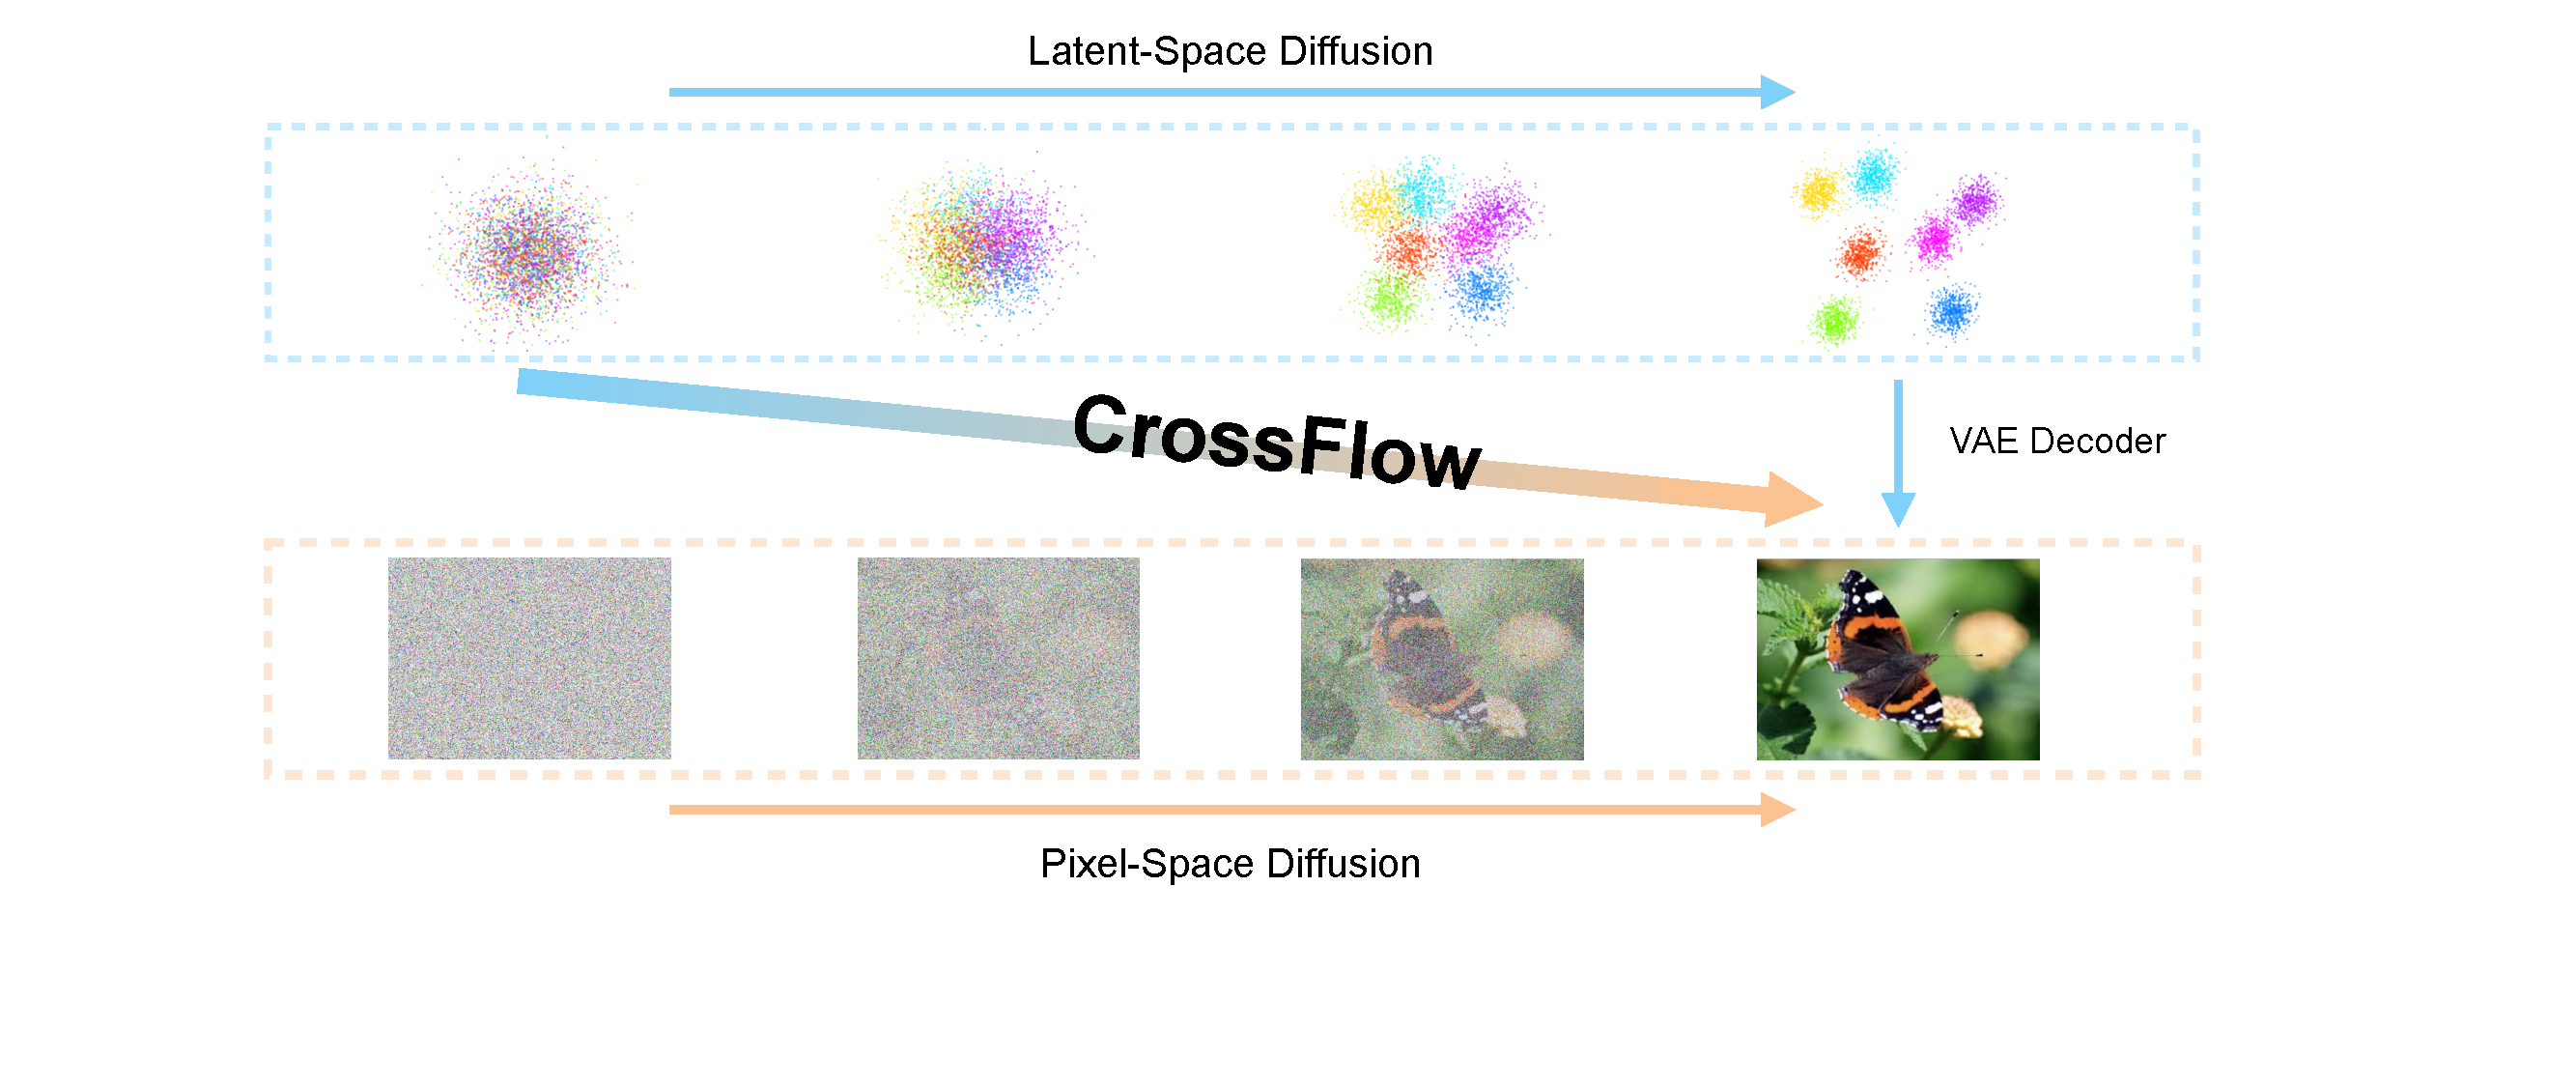
\includegraphics[width=0.9\linewidth]{imgs/CrossFlow_fig1.pdf}
    \caption{\textbf{CrossFlow generation paradigm.} Latent diffusion uses a two-stage pipeline: iterative denoising in latent space followed by VAE decoding. Pixel-space diffusion performs iterative denoising directly in the image domain. CrossFlow uses a single model to map a noisy latent prior directly to a pixel-space image, unifying one-step generation and latent-to-pixel decoding.}
    \label{fig:crossflow_paradigm}
\end{figure}

This paper asks a simple question: must the noise space and the output space be the same? A useful image generator could start from a latent prior, preserve the computational advantages of latent representations, and still predict the image itself. Such a model would remove the explicit decoder stage, train directly on generated images, and expose the model during training to the kind of noisy or imperfect latents that appear during generation.

We propose \emph{CrossFlow}, a cross-space one-step generation framework. As shown in Figure~\ref{fig:crossflow_paradigm}, CrossFlow maps a noisy latent input directly to a pixel-space image in a single function evaluation. This setting is different from standard flow matching, where the model predicts a velocity to update the current state, both of which must live in the same space. A latent-to-pixel model cannot update a latent variable with a pixel-space velocity. CrossFlow resolves this mismatch by deriving objectives in which the latent-space velocity is eliminated from the supervised target. The latent path still defines how clean latents are corrupted, but the network output is pixel.

% The derivation leads to two practical requirements. First, the loss cannot require the model to predict a latent-space velocity. Second, the model output must represent the image itself, rather than a quantity that is linearly combined with the latent input. These requirements yield a family of velocity-free cross-space objectives. We focus on a reconstruction-compatible branch that anchors the prediction to the clean image and propagates that image-level constraint along the noisy latent trajectory through a time-derivative term. A consistency-like branch is possible, but our diagnostic and ablation results show that the reconstruction-compatible branch is substantially more reliable.

We instantiate CrossFlow with a fixed pretrained image encoder and a Vision Transformer generator. During training, an image is encoded into a latent, corrupted along a latent trajectory, and passed to the generator, which directly predicts pixels. Because the output is already an image, we can use reconstruction, perceptual, and adversarial losses in the same training objective. The resulting model has two uses: it is a one-step latent-to-pixel generator, and it can replace the decoder in a latent diffusion pipeline whose latents are produced by a generator rather than by a clean encoder. On ImageNet-1k at $256\times256$, CrossFlow-B, CrossFlow-L, and CrossFlow-XL achieve 2.54, 1.69, and 1.62 FID, respectively, with one function evaluation. CrossFlow-XL is competitive with strong multi-step latent diffusion baselines while operating in a different regime: it maps latent noise directly to pixels and does not use a separate decoder at inference. Ablations show that both the latent representation and pixel-space auxiliary losses matter. CrossFlow also improves FID when used as a decoder for latents produced by a DiT generator in the VA-VAE latent space.

Our contributions are:
\begin{itemize}
    \item We introduce CrossFlow, a one-step generation framework in which the input prior and output image may live in different representation spaces.
    \item We implement CrossFlow as a ViT-based latent-to-pixel generator with direct pixel-space perceptual and adversarial refinement.
    \item We show strong one-step ImageNet $256\times256$ generation results and demonstrate that the same model can replace a VAE decoder for generated latents.
\end{itemize}
